\documentclass[10pt,a4paper,ssfamily]{exam}
\usepackage[numbers,sort&compress]{natbib}
\usepackage[utf8]{inputenc}
\usepackage[brazil]{babel}
\renewcommand{\baselinestretch}{1.15}
\usepackage{epsfig}
\usepackage{nicefrac}
\usepackage{graphicx}
\usepackage{makeidx}
\usepackage{multicol}    
\usepackage{multirow}
\usepackage{amssymb}
\usepackage{enumitem}
\usepackage{xcolor}
\usepackage{lmodern}
\usepackage{scrextend}
\usepackage{xcolor}
\usepackage[hidelinks]{hyperref}
\usepackage{amsmath}
\usepackage{mathtools}
\usepackage{chemformula}
\usepackage{mhchem}
\renewcommand{\t}{\text}
\newcommand{\listfont}{\bf\fontencoding{OT1}\sffamily\large}
\newcommand{\titlesfont}{\fontencoding{OT1}\sffamily\large}
\renewcommand{\baselinestretch}{1.24}
\newcommand{\oC}{$^\circ$C}
\newcommand{\sen}{\textrm{sen }}
\newcommand{\Mg}{Mg$^{2+}$}
\newcommand{\sol}[1]{\href{http://leandro.iqm.unicamp.br/shtml/didatico/qf935/atividades/#1.f90}{Solução}}
\newcommand*{\LargeCdot}{\raisebox{-0.25ex}{\scalebox{1.2}{$\cdot$}}}

% Activity envinronment

\newsavebox{\fmbox}
\newenvironment{ex}
{\begin{center}\vspace{0.3cm}\begin{lrbox}{\fmbox}\begin{minipage}{12cm}{\bf Atividades}
\begin{enumerate}\setcounter{enumi}{\exnumber}}
{\global\chardef\exnumber=\value{enumi}\end{enumerate}\end{minipage}\end{lrbox}\fbox{\usebox{\fmbox}}\vspace{0.3cm}\end{center}}

% Code blocks definitions

\usepackage{listings}

\renewcommand{\t}{\textrm}
\lstnewenvironment{code}{\lstset{language=[90]Fortran,
  basicstyle=\ttfamily,
  keywordstyle=\color{blue},
  commentstyle=\color{gray},
  identifierstyle=\color[RGB]{0,102,0}\textbf,
  xleftmargin=1.5cm,
  showstringspaces=false,
  morecomment=[l]{!\ }% Comment only with space after !
}}{}

\lstdefinestyle{code}{
  language=[90]Fortran, 
  basicstyle=\ttfamily,
  keywordstyle=\color{blue},
  commentstyle=\color{gray},
  identifierstyle=\color[RGB]{0,102,0}\textbf,
  xleftmargin=1.5cm,
  showstringspaces=false,
  morecomment=[l]{!\ }% Comment only with space after !
}
\newcommand{\codefile}[1]{\lstinputlisting[style=code]{#1}
            \begin{center}
            \href{http://leandro.iqm.unicamp.br/leandro/shtml/didatico/simulacoes/#1}
                 {\textcolor{blue}{[Clique para baixar o código]}}
            \end{center}}

\newcommand{\codelink}[1]{
            \begin{center}
            \href{http://leandro.iqm.unicamp.br/leandro/shtml/didatico/simulacoes/#1}
                 {\textcolor{blue}{[Clique para baixar o código]}}
            \end{center}}

\begin{document}

\pagestyle{plain}

% Start exercise counter
\global\chardef\exnumber=0

\sffamily

\pagestyle{empty}


\begin{center}
{\bf\Large Fundamentos Computacionais de Simulações em Química}

Leandro Martínez\\
leandro@iqm.unicamp.br \\
Última atualização: \today
\end{center}

\tableofcontents

\section{Elementos básicos de programação}

A linguagem de escolha do curso é o Fortran, nas suas versões mais
recentes (isto é, a partir de Fortran90). A escolha desta linguagem se
deve à simplicidade de sua sintaxe e à eficiência numérica dos programas
gerados. Fortran é uma linguagem idealizada, desde o princípio, para a
computação numérica. Por esta razão, não é a linguagem mais flexível,
mas é a que permite a geração de códigos dependentes de computação
numérica de alto desempenho com maior facilidade. 

Há inúmeros cursos, tutoriais e livros sobre Fortran. Uma busca na
internet por ``Introdução ao Fortran'', em qualquer idioma, permite o
acesso a uma grande variedade de material gratuito. Este curso, no
entanto, não é um curso de Fortran. Este é um curso de fundamentos de
simulação. As simulações requerem uma linguagem de programação, e o
Fortran é a linguagem de escolha, porque sua sintaxe é simples e
natural. Espera-se que o aluno aprenda a linguagem de programação com
exemplos e resolvendo problemas (como eu aprendi). Nenhuma importância
será dada a estruturas de linguagem e programação exceto no momento em
que sejam requeridas. Ao final do curso, espera-se que o aluno adquira
uma razoável familiaridade com a programação como conceito e com a
linguagem, e possa buscar as ferramentas corretas para a resolução de
seus próprios problemas aplicados.  

\subsection{Estrutura básica do programa}

Antes de nada, tudo o que compuser o os programas será escrito em
inglês. Há duas razões para isto. A mais direta, e banal, é que no
inglês não há acentos, e acentos são uma fonte de problemas em um
programa. A segunda é que é um hábito saudável se acostumar a programar
tudo pensando que, um dia, o programa será distribuído para outras
pessoas, e o inglês é a língua para isso hoje em dia.

A estrutura mínima de um programa consiste em:
\begin{code}
program test
  ! This is a commentary
end program test
\end{code}
Todas as linhas que começam com uma exclamação, "!" são ignoradas, sendo
chamadas de ``comentários''. Os comentários ajudam, em programas
complexos, a entender o que está sendo feito.

Para as pessoas que estão usando o compilador para Windows recomendado
neste curso ({\tt Force 2.0}) , é necessário acrescentar ao fim do
programa uma pergunta para que a janela em que o programa é executado
não se feche antes que possamos ver o que aconteceu. Neste caso, o
programa mínimo sugerido é: 
\begin{code}
program test
  write(*,*) 'End program?'
  read(*,*) 
end program test
\end{code}
Este programa vai simplesmente fazer a pergunta e esperar uma resposta.
A resposta pode ser qualquer coisa, mesmo apenas um ``Enter''.
Precisamos disso, no Windows, para que possamos ver o que aconteceu
antes, ou a janela que será aberta pelo programa fechará
instantaneamente quando o programa termine (teste os dois casos). Por
hora, não nos preocupemos com os {\tt (*,*)}. Quando for necessário
explicar o que é isso, o faremos.

A representação dos números, no computador, tem limitações. Um número
inteiro ocupa uma determinada quantidade de bits na memória. Um número
inteiro, no computador, não é {\it qualquer} número inteiro, é um número
inteiro que pode ser representado pela quantidade de bits que foi
escolhida para isso. Em Fortran, é necessário avisar que tipo de número
está sendo usado. Esse aviso se chama ``declaração''. A declaração de um
número inteiro se faz com:
\begin{code}
integer :: i
\end{code}  
Um valor pode ser atribuído à variável e, em seguida, escrito na tela,
usando, por exemplo:
\begin{code}
i = 571
write(*,*) i
\end{code}
Como o número ocupa um espaço finito na memória, há um número máximo que
pode ser representado. Se o programa tentar atribuir um número maior que
esse à variável inteira, algo estranho deve acontecer.

\begin{ex}
\item
Descubra qual é o maior número inteiro que pode ser representado com a
declaração padrão acima.
\end{ex}

Da mesma forma, números reais podem ser definidos. No entanto, podem ser
definidos facilmente com diferentes precisões:
\begin{code}
real :: a
double precision :: b  
\end{code}

\begin{ex}
\item
Atribua valores distintos às variáveis {\tt a} e {\tt b}, como
declaradas acima, e verifique quantos algarismos significativos possuem.
\end{ex}

A precisão finita dos números, no computador, faz com que as operações
aritméticas tenham limitações. Por exemplo, o valor de {\tt b} pode ser
somado a {\tt a} com
\begin{code}
  a = a + b 
  write(*,*) a
\end{code}
Se a relação entre as ordens de grandeza dos dois números for maior que
a precisão com que {\tt a} é armazenado no computador, esta soma ``dá
errado''.
\begin{ex}
\item
Atribua o valor $1.$ para {\tt a}. Atribua valores diferentes para {\tt
b}, com muitas ordens de grandeza diferentes, e escreva o resultado da
soma de {\tt a} com {\tt b}. 
\end{ex}
Um caso particular importante desta limitação de precisão aritmética é o
da soma de muitos números de ordens de grandeza diferentes. Por exemplo,
podemos atribuir o valor $1\times 10^8$ para {\tt a}, fazendo a seguinte
operação (aqui introduzimos o primeiro {\it loop}):
\begin{code}
program sum_a
  integer :: i
  real :: a 
  a = 0.
  do i = 1, 10000
    a = a + 1.e-4
  end do
  write(*,*) a
end program sum_a
\end{code} 
Este programa soma dez mil vezes o número $10^{-4}$. O resultado deve
ser $1.$, exceto devido a imprecisões numéricas. 
\begin{ex}
\item
Antes de iniciar o loop acima, some $10^4$ a {\tt a}. Verifique o
resultado do programa.
\item
Depois de finalizado o loop acima (sem a modificação do item
anterior), some os mesmos $10^4$ a {\tt a}, e verifique o resultado.
compare com o resultado do item anterior.
\end{ex}
Você deve ter notado que os resultados das somas são diferentes,
dependendo da ordem em que elas são feitas. É importante ter isto em
mente sempre que operações envolverem números com muitas ordens de
grandeza de diferença. 

Há várias maneiras de escrever um loop em Fortran. Uma maneira
muito útil é a que usa o conceito de ``enquanto'',
\begin{code}
a = 0.
do while( a < 1. )
  a = a + 1.e-3
end do
\end{code}
\begin{ex}
\item
Você já deve ter verificado o que acontece com um número inteiro quando
tenta-se ultrapassar o valor máximo representável. Use a estrutura do
loop acima para escrever o inteiro máximo representável.
\end{ex}

Loops podem também ser parados por testes feitos internamente. Por
exemplo, a seguinte sintaxe é válida:
\begin{code}
i = 0
do 
  i = i + 1
  if ( i > 10 ) then
    exit
  end if
end do
\end{code}

O loop não possui nenhum teste, e só termina quando o o teste realizado
internamente se satisfaz. Este tipo de saída de um loop vai ser muito
útil nas simulações, em particular para a checagem de erros.  

\newpage
\section{Primeiras simulações: cinética química}
\label{sims}

Aqui estudaremos a simulação de uma cinética de primeira ordem,
irreversível, na forma
\[
\ch{A} \xrightarrow{k_1} \ch{B}
\]
A equação diferencial que determina como a concentração de A varia
no tempo é
\[
-\frac{d[\ch{A}]}{dt} = k_1[\ch{A}]
\]
Dada uma concentração inicial $[\ch{A}](0)$, podemos calcular uma
aproximação da concentração em um tempo posterior, usando
\[
[\ch{A}](\Delta t) = [\ch{A}](0) + \frac{d[\ch{A}]}{dt}\Delta t
\]
ou seja,
\[
[\ch{A}](\Delta t) = [\ch{A}](0) - k_1[\ch{A}](0)\Delta t
\]
O resultado desta conta nos dá um novo valor de concentração, 
que permite que calculemos a concentração em um instante mais avançado
no tempo. A fórmula geral deste processo é
\begin{equation}\label{discret1}
[\ch{A}](t + \Delta t) = [\ch{A}](t) - k_1[\ch{A}](t)\Delta t
\end{equation}
O programa abaixo faz este procedimento recursivamente, até que a
concentração do reagente A se anule. Estude o programa com
atenção:

\codefile{./codes/sim1.f90}

Aqui criamos pela primeira vez um arquivo de saída para nosso programa.
Ele se chama {\tt sim1.dat}, e a ele foi atribuída a ``unidade {\tt
10}''. Quando escrevemos o resultado, o {\tt write} foi modificado para
escrever o tempo e a concentração na ``unidade {\tt 10}'', ou seja, nesse
arquivo. Esse arquivo pode ser importado em qualquer programa de fazer
gráficos, para vermos o que está acontecendo.

\begin{ex}
\item
Varie os valores de {\tt CA}, {\tt k1} e {\tt dt} no programa acima, e
observe o comportamento da concentração em função do tempo em cada caso.
Se necessário, varie {\tt nsteps} também.
\item
Um dos resultados possíveis da execução do programa acima, é a obtenção
de concentrações negativas para o reagente A. Naturalmente, isso se deve a um erro
numérico. Adicione um ``{\tt if ... end if}'' ao programa que detecte esse erro,
escreva uma mensagem de erro, e pare o programa.
\item
Adicione ao programa o cálculo da concentração do produto B. Assuma que
a concentração de B tem um valor inicial especifico. Escreva também a
concentração de B no arquivo de saída. 
\item
Nós sabemos que a solução analítica da equação diferencial deste
problema é simplesmente $[\ch{A}(t)]=[\ch{A}](0)e^{-k_1 t}$. Em Fortran, essa
exponencial se escreve como {\tt exp(-k1*t)}. Escreva o resultado da
solução analítica em seguida de CA, no programa, e veja que diferença
tem a solução analítica da solução numérica, em cada tempo, em função
dos parâmetros {\tt CA}, {\tt k1} e {\tt dt}. 
\end{ex}

É relativamente fácil lidar com o aumento da complexidade do mecanismo
reacional em uma simulação de cinética química. A reação reversível, 
\[
\ch{A} \xrightleftharpoons[k_{-1}]{k_1} \ch{B}
\]
tem duas constantes de velocidade, e as equações diferenciais que regem
o comportamento das concentrações de A e B são, agora, dependentes
destas duas velocidades. Ou seja, agora temos duas equações diferenciais
que regem a evolução temporal das concentrações:
\[
-\frac{d[{\t A}]}{dt} = k_1[{\t A}] - k_{-1}[{\t B}]
\]
\[
\frac{d[{\t B}]}{dt} = k_1[{\t A}] - k_{-1}[{\t B}]
\]
\begin{ex}
\item
Escreva a {\it discretização} de cada uma destas equações, seguindo o
exemplo da Equação~\ref{discret1}.
\end{ex}
Há duas maneiras de programar a evolução temporal das concentrações das
espécies. Uma delas propaga as concentrações usando as discretizações na
forma da Equação~\ref{discret1} para ambas as espécies. A outra é usar
um balanço de massa, já que sabemos que existe uma relação entre as
concentrações. Neste caso, $[{\t A}] + [{\t B}] = [{\t A}]_0 + [{\t
B}]_0$. O programa usando o balanço de massa pode ser:

\codefile{./codes/sim2.f90}

Entenda bem o programa acima. Note que, agora, salvamos as concentrações
iniciais em duas novas variáveis, {\tt CA0} e {\tt CB0}, porque são
usadas o tempo todo no cálculo da concentração de B pelo balanço de
massa. Um detalhe: no início do programa, adicionamos um comando {\tt
implicit~none}. Este comando serve para que não esqueçamos de declarar
nenhuma variável. Se uma variável, como {\tt CA}, {\tt time}, etc, for
usada, mas seu tipo não tiver sido declarado, a compilação do programa
vai acusar um erro. Na medida que o programa for ficando grande, isto
vai ser importante. Portanto, a partir de agora, todos os nossos
programas começarão com esse comando.  
\begin{ex}
\item
O programa acima pode ser modificado para calcular a concentração de
B usando a discretização da equação diferencial correspondente em vez do
balanço de massa. Faça isso.
\item
Com esta modificação, é possível testar a precisão da propagação das
concentrações já que, em princípio, deveriam satisfazer sempre o balanço
de massa. Se não satisfazem, isto quer dizer que há algo que não
está indo bem. Calcule o erro no balanço de massa ao longo da execução
do programa, e escreva este erro. Estude como este erro varia em função
do passo de tempo e das constantes de velocidade. 
\item
Você terá percebido que sempre há um erro associado à propagação das
concentrações. Modifique seu programa adicionando um teste ({\tt if...})
que detecte quando o erro for grande demais. 
\end{ex}

Não há nada fundamentalmente diferente do que fizemos até aqui para a
simulação da cinética de nenhum sistema químico. Basta escrever e
discretizar as equações diferenciais correspondentes ao mecanismo
reacional proposto, e programar a integração numérica das equações.    
\begin{ex}
\item
O mecanismo-modelo mais conhecido de catálise enzimática é o mecanismo
de Michaellis-Menten, 
\[
\ch{E + S} \xrightleftharpoons[k_f]{k_r} \ch{ES} \xrightarrow{k_{cat}} \ch{E + P}
\]
onde E e S são a enzima e o substrato, ES é o complexo enzima-substrato,
e P é o produto da reação. Faça um programa que simule esta cinética
enzimática. Varie as concentrações dos reagentes para encontrar as
condições nas quais a aproximação do estado estacionário é razoável
(isto é, que a concentração do complexo é aproximadamente constante ao
longo da reação).    
\item
A decomposição da camada de ozônio pelos clorofluorcarbonos acontece
através de uma reação em cadeia. A reação se inicia pela decomposição do
clorofluorcarbono formando cloro radicalar, o que acontece sob radiação
ultravioleta,
\[
\ch{CFCl_3} \xrightarrow{} \ch{Cl^. + ^.CFCL_2}
\]
O cloro radicalar decompõe o ozônio de forma catalítica, pelas reações
\[
\ch{Cl^. + O_3} \rightarrow \ch{ClO + O_2}
\]
\[
\ch{ClO + O_3} \rightarrow \ch{Cl^.} + 2\ch{O_2}
\]
Faça um programa que simule este mecanismo reacional.
\end{ex}

\newpage
\section{Otimização com derivadas}

Quase todo problema real envolve a maximização ou minimização de alguma
coisa. Falemos de Química. Quando sintetizamos um novo composto,
tentamos maximizar o rendimento. Quando criamos um novo material,
tentamos melhorar algumas de suas características que nos interessam,
como, por exemplo, a eficiência de uma célula solar, ou a resistência de
um polímero. Quando fazemos um ajuste de uma curva experimental, estamos
encontrando qual a equação (linear ou não) que melhor se ajusta às
observações. Na química teórica, permanentemente estamos minimizando
energias para obter estruturas químicas melhores e, com sorte, mais
representativas das estruturas reais.     

A otimização, do ponto de vista da computação, se divide em duas grandes
áreas: otimização com o uso de derivadas, e otimização sem o uso de
derivadas. As derivadas de uma função indicam para onde esta função
cresce, portanto consistem em uma informação importantíssima, se
disponível, na resolução de um problema de otimização. As derivadas de
uma função são conhecidas, no entanto, somente quando conhecemos,
explicitamente, a a função em si. Quando não conhecemos a função, temos
que otimizar sem derivadas. Por exemplo, se queremos minimizar a função
$f(x)=x^2$, podemos usar a informação sobre sua derivada, $df/dx=2x$. No
entanto, se queremos maximizar a resistência de um compósito variando
sua composição, não temos a derivada, porque não conhecemos a {\it
função} que nos dá a resistência como função da composição. Vamos
aprender, agora, os conceitos básicos da minimização com e sem
derivadas, e veremos que muitos problemas reais podem ser modelados
usando uma ou outra técnica.  

\subsection{Minimizando com derivadas}

Vamos construir um programa, o mais simples possível, que procure usar a
informação da derivada de uma função para encontrar seu mínimo valor.
Tomemos a função
\[
f(x) = x^2,
\]
cuja derivada é
\[
\frac{df}{dx} = 2x
\]
Nós sabemos que o mínimo desta função está em $x=0$. O que nos interessa
aqui é como um tal problema é abordado do ponto de vista numérico.

A derivada indica para que lado a função cresce, portanto ``menos a
derivada'' indica para que lado ela diminui. O programa mais simples que
tenta obter o mínimo da função é aquele que simplesmente testa a função
em vários pontos, na direção indicada pela derivada, e para se a função
simplesmente sobre. Testar a função na direção indicada pela derivada
significa usar uma aproximação da função. Por exemplo, a aproximação de
Taylor de primeira ordem,
\begin{equation}\label{min1}
f(x_1) \approx f(x_0) + f'(x_0) (x_1 - x_0)
\end{equation}
onde $f'(x_0)$ é a derivada de $f(x)$ calculada no ponto $x_0$.
Portanto, o processo de busca do mínimo da função vai consistir em
testar pontos $x_1$ diferentes, na direção em que a derivada indica que
o mínimo deve estar. A direção da derivada, no caso unidimensional, é
apenas seu sinal, isto é, se ela indica se a função cresce na direção de
$x$ mais positivo, ou negativo. Portanto, o passo em $x$ é dado na
direção
\[
-\frac{f'(x_0)}{|f'(x_0)|}
\]  
que pode valer $+1$ ou $-1$. Este caso é muito simples, mas se a função
tivesse mais dimensões, a direção seria dada por $-\nabla f/|\nabla f|$,
e seria um vetor unitário na direção da derivada. Faremos isso mais
tarde. O código abaixo implementa esta estratégia
({\tt dabs(x)} é o módulo do número $x$):

\codefile{./codes/min1.f90}

O código acima possui muitas das características essenciais de qualquer
programa de simulação, ou otimização. O programa se inicia atribuindo
valores inciais para as variáveis ($x$) e os parâmetros que serão
usados. Neste caso, o método envolve um único parâmetro, $\Delta x$, que
é o tamanho do ``passo'' que vai ser dado na direção da derivada
decrescente (a diferença $x_1-x_0$ da Equação\ref{min1}). Dentro do
loop calcula-se a derivada, e modifica-se o valor de $x$ na direção da
derivada, com passo $\Delta x$, i. e., $x=x-f'(x)\Delta x$. Testamos, em
seguida, se a função aumentou o diminuiu. Se diminuiu, o novo $x$ é
salvo como o melhor $x$ até o momento. Se aumentou, decretamos que o
programa terminou.  

\begin{ex}
\item
Varie o valor de $\Delta x$ no programa acima, e estude o que acontece.
Qual a precisão das soluções atingidas. Que resultados inesperados podem
acontecer? Por quê? O que ocorre se o passo $\Delta x$ for muito grande? 
\item
Modifique o programa de tal forma que quando a função aumenta, em vez de
parar, simplesmente continua-se, mas sem salvar o melhor ponto $x$. Estabeleça
um limite de número de voltas no loop, porque agora o programa poderá ficar
rodando para sempre. Observe o que acontece com a variação do passo
$\Delta x$, em particular para passos grandes.
\item
Faça um programa que minimize a função $x^2+\sen(10x)$. A sintaxe
para o seno em dupla precisão é {\tt dsin(x)}. Faça testes variando o tamanho de
passo e os pontos iniciais, no intervalo $[-2,2]$. 
\item\label{min2}
Uma alternativa razoável para o passo $\Delta x$ é que ele seja
proporcional à derivada. Ou seja, se a derivada é grande, dá-se um passo
grande, se é pequena, dá-se um passo pequeno em $x$. Para isso, basta
eliminar a normalização da direção da derivada. Faça isso no programa
{\tt min1}, e avalie as características do processo de minimização
(número de iterações até o fim e precisão da solução).
\end{ex}

O passo que faz o algoritmo de otimização mais robusto é o passo que
varia de forma inteligente de acordo com o que acontece com a função.  A
maior parte dos métodos de otimização usam alguma coisa similar ao que
vamos descrever agora.

A ideia consiste em mover as variáveis na direção desejada (neste caso,
na direção contrária à derivada) e, antes de {\it aceitar} o novo ponto,
{\it testar} se a função aumento ou diminuiu. Se a função diminuiu, que
é o que queremos, a direção em que andamos é boa e, talvez, possamos
aumentar o passo. Além disso, aceitamos o novo ponto. Se a função
aumentou, o que não queremos, não aceitamos o novo ponto, e reduzimos o
passo para ficarmos mais próximos do ponto atual. Estas ideias estão
associadas ao fato de que estamos nos movendo nas variáveis usando uma
aproximação de Taylor. A aproximação de Taylor é boa próxima do ponto {\it
corrente}. Se o passo for suficientemente pequeno, a função tem que
diminuir se a derivada assim o diz. Se o passo for grande demais a
função pode aumentar, porque a aproximação é ruim longe do ponto em que
foi feita. 

O programa, então, tem que ser modificado, para introduzir este passo de
tamanho variável. Fundamentalmente, temos que introduzir alguns testes,
e um critério para a variação do passo $\Delta x$: 
\begin{code}
...
if ( ftrial < f ) then
  deltax = deltax * 2.d0
  f = ftrial
  x = xtrial
else
  deltax = deltax / 2.d0
end if
...
\end{code}
O ponto é que, agora, antes de modificar efetivamente a variável $x$,
vamos modificar outra variável, $x_\text{trial}$, e testar o que
acontece com o valor dessa função nesse ponto teste. Dependendo de como
varia a função, tomamos uma decisão sobre a atualização do ponto
corrente $x$ e outra sobre o tamanho do passo na iteração seguinte. Note
que, agora, o valor da função sempre vai diminuir em pontos {\it
aceitados}, portanto temos que definir um critério para parar o
programa. Um critério razoável é, por exemplo, o valor da derivada. Se
ela for muito pequena, podemos considerar que chegamos em um ponto
crítico da função.

\begin{ex}
\item
Modifique o programa do exercício~\ref{min2}, introduzindo as
modificações discutidas nesta parte. Várias modificações devem ser
feitas no programa, e é importante entender o que está se fazendo antes
de modificar o programa. A solução está na lista de soluções. Mas tente
bastante antes de olhar lá. Vale a pena. 
\item
Compare o programa da atividade anterior com o programa da
atividade~\ref{min2} quanto à eficiência em encontrar uma solução. A
eficiência, neste caso, é composta pelo número de {\it iterações}, e
pelo valor final da função.
\end{ex}

\subsection{Funções de múltiplas variáveis}

Agora vamos modificar o programa para trabalhar com funções de mais de
uma variável. Neste caso, a direção de aumento da função é dada pelo
gradiente da função, um vetor. Tomemos a função $f(x,y)=x^2+y^2$, por
exemplo. Seu gradiente é o vetor
\[
\nabla f = \begin{bmatrix} 
              \partial f/\partial x \\
              \partial f/\partial y 
           \end{bmatrix} =
           \begin{bmatrix} 
              2x \\
              2y 
           \end{bmatrix}
\]
Portanto, mover o ponto $(x,y)$ na direção de decréscimo da função
significa mover cada uma das suas variáveis nessa direção,
\[
x_\text{trial} = x - \frac{\partial f}{\partial x}(x) \Delta x 
\]
\[
y_\text{trial} = y - \frac{\partial f}{\partial y}(y) \Delta y
\]
Em geral, usamos o mesmo passo básico, $\Delta s$ para as duas variáveis, e podemos
escrever as equações acima na forma
\[
\begin{bmatrix} x \\ y \end{bmatrix}_\text{trial} =
\begin{bmatrix} x \\ y \end{bmatrix} - 
\begin{bmatrix} \partial f / \partial x \\ \partial f / \partial y
\end{bmatrix} \Delta s.
\]
Esta mesma equação pode ser escrita de forma genéria e sucinta usando
notação vetorial,
\[
\vec{x}_\text{trial} = \vec{x} - \nabla f \Delta s
\]
O programa pode minimizar a função $x^2+y^2$ usando o mesmo procedimento
que foi usado para as funções de uma variável. Calcula-se um
$\vec{x}_\text{trial}$, testa-se se a função diminui. Se a função
diminui, aceita-se $\vec{x}_\text{trial}$ como o novo $\vec{x}$ e
aumenta-se o passo $\Delta s$. Em caso contrário, diminui-se $\Delta s$.
\begin{ex}
\item
Modifique o programa da atividade 21 para minimizar a função $x^2+y^2$. Agora, em
lugar da derivada, temos um gradiente. Em lugar do módulo da derivada
como critério de parada, temos a norma do gradiente. 
\end{ex}
Usando a notação vetorial, definimos que a função é dependente dos
elementos do vetor $\vec{x}$, que chamaremos $x_1$ e $x_2$. No programa,
um vetor é declarado usando
\begin{code}
double precision :: x(2)
\end{code}
e, em lugar de usar duas variáveis, {\tt x} e {\tt y}, usaremos as
componentes do vetor {\tt x(1)} e {\tt x(2)}.
\begin{ex}
\item
Modifique o programa anterior para usar a notação vetorial, em lugar de
definir uma variável diferente para cada variável do problema.
\item
Modifique o programa anterior para minimizar a função $x^2 + y^2 + z^2$. 
\item
Modifique o programa anterior para minimizar a função $x_1^2 + x_2^2 +
\dots + x_{1000}^2$.
\end{ex}

\section{Subrotinas e funções}

Os nossos programas estão ficando complicados, e você já deve ter percebido
que estamos começando a repetir muitas coisas. Para aproveitar os
programas feitos antes, e evitar erros cada vez que algo novo vai ser
feito, foram inventadas as {\it subrotinas} e as {\it funções}. 

As funções você já conhece. Quando você usa a notação, por exemplo {\tt
dabs(x)}, que calcula o módulo de $x$, você ``chamou'' a função módulo.
Essa função está escrita em algum lugar, e deve ser alguma coisa assim:
\begin{code}
function dabs(x)
  implicit none
  double precision :: x
  if ( x > 0 ) then
    dabs = x
  else
    dabs = -1.d0*x
  end if
end function dabs
\end{code}
Entenda este exemplo. O valor de $x$ é um {\it parâmetro de entrada} da
função. A função {\it retorna} o valor do módulo de $x$ em {\tt dabs}.
Esta função poderia estar escrita no mesmo arquivo em que está o seu
programa, depois do fim do programa.
\begin{ex}
\item
Faça um programa que, dado um valor de uma variável $x$, chame uma
função que multiplique o valor dessa variável por cinco.
\item
Faça um programa que calcule a soma do quadrado dos elementos de um
vetor. O vetor pode ser passado como parâmetro da função de uma vez só.
Cuidado com as declarações das variáveis, elas devem ser declaradas
dentro e fora das das funções, da mesma forma.
\end{ex}

O próximo passo é aproveitar esta estrutura de funções e subrotinas para
estruturar o nosso programa de minimização. Vamos criar agora subrotinas
que calculam o valor da função e o gradiente, em cada ponto testado. A
subrotina que calcula a função pode ser (poderia ser uma função também):
\begin{code}
subroutine computef(n,x,f)
  implicit none
  integer :: i, n
  double precision :: x(n), f
  f = 0.d0
  do i = 1, n
    f = f + x(i)**2
  end do
end subroutine computef
\end{code}
Os parâmetros {\tt n} e {\tt x} são {\it parâmetros de entrada} da
subrotina, e {\tt f} é o parâmetro de saída (isto não tem a ver com a a
ordem dos parâmetros, é apenas uma observação lógica). 
A subrotina que calcula o gradiente é:
\begin{code}
subroutine computeg(n,x,g)
  implicit none
  integer :: i, n
  double precision :: x(n), g(n)
  do i = 1, n
    g(i) = 2.d0*x(i)
  end do
end subroutine computeg
\end{code}

Estas duas subrotinas podem ser colocadas antes ou depois do programa
principal, no mesmo arquivo, ou podem ser colocadas em outros arquivos.
No programa principal, em lugar de calcular explicitamente a função ou
o gradiente, usa-se
\begin{code}
call computef(n,x,f}
\end{code}
e
\begin{code}
call computeg(n,x,g)
\end{code}
Nos nossos programas calculamos um ponto teste, que chamamos {\tt
xtrial}. As subrotinas podem ser {\it chamadas} usando este vetor, por
exemplo,
\begin{code}
call computef(n,xtrial,f)
\end{code} 
Ou seja, não é necessário programar explicitamente nenhuma outra vez a
função que está sendo minimizada. Basta chamar a subrotina adequada.
Note que, com isto, modificar o programa para minimizar uma função
diferente passa a ser, essencialmente, mudar a subrotina, e programa
principal pode ser sempre o mesmo. Se a subrotina for colocada em um
arquivo diferente do programa principal, é necessário compilar tudo
junto. Na linha de comando, isto é bastante simples, por exemplo:
\begin{center}
{\tt gfortran -o minimize min2.f90 computef.f90 computeg.f90}
\end{center}
onde {\tt minimize} é o nome do executável que será gerado, e os
arquivos que seguem contém o programa principal e cada uma das
subrotinas (no Windows é necessário usar o Prompt de comando e colocar o
compilador no {\it PATH}, peça ajuda se precisar). Note que, se quiser
criar um programa para minimizar outra função, basta criar as subrotinas
em outros aquivos, com outros nomes, e compilar de acordo. 
\begin{ex}
\item
Modifique o programa do exercício 26 introduzindo subrotinas para o
cálculo da função e do gradiente.
\item
Crie subrotinas distintas para o cálculo da função e do gradiente de
outras funções, por exemplo, $(x_1-1)^4+(x_2-3)^2+(x_3+7)^4$, ou
$x_1^4\sen(x)+x_2^2$. Ou qualquer outra que desejar.
\end{ex}

\section{Minimização sem derivadas}

A minimização sem derivadas é, conceitualmente, mais simples que a
minimização com derivadas. A vantagem é que, naturalmente, nem sempre
sabemos calcular a derivada da função que desejamos otimizar, ou a
derivada pode nem mesmo existir. Portanto, a otimização sem derivadas é
sempre uma maneira de caminhar sobre a função, avaliando diferentes
pontos, procurando otimizar a função. Sem saber a derivada, não sabemos
para onde a função aumenta ou diminui, portanto, os novos pontos
testados serão sempre menos ``racionais'' que quando conhecemos as
derivadas. Naturalmente, isto é muito pior. Não saber para onde a função
aumenta é uma grande desvantagem e, portanto, sempre que for possível
usá-las, devem ser usadas.

O método de otimização sem derivadas mais simples consiste em testar,
aleatoriamente, novos pontos, e ficar com o melhor. 

\subsection{Gerador de números aleatórios}

Nos métodos de otimização sem derivadas, e em muitas outras
situações, vamos precisar gerar números aleatórios. Todas as linguagens
possuem alguma função que gera números que {\it parecem} aleatórios. Em
Fortran, o gerador de números aleatórios se usa da seguinte maneira:  
\begin{code}
double precision :: random
call random_number(random)
\end{code}
O número real {\tt random} terá um valor aleatório, no intervalo entre 0
e 1. Uma segunda chamada, em seguida, da mesma subrotina, vai gerar {\it
outro} número aleatório entre 0 e 1.
\begin{ex}
\item
Faça um programa que gere vários números aleatórios em sequência, e
observe os valores gerados. 
\item
Faça um programa que gere milhares de valores aleatórios, e faça um
gráfico destes valores, para verificar, visualmente, a natureza de sua
aleatoriedade.
\end{ex}

\subsection{Minimizando $x^2+y^2$}

Vamos fazer alguns programas para minimizar a função $x^2 + y^2$, sem
usar derivadas, com diferentes graus de sofisticação. O primeiro
programa é muito simples, e consiste em testar pontos aleatoriamente. O
fundamental aqui é {\it preservar o melhor valor}. Não há escolha de
como parar o programa a não ser por excesso de tempo. Isto é, a busca
pelo minimizador para quando cansamos de fazer a busca. 
\codefile{./codes/randomsearch.f90}
Note as seguintes características do programa: 1) Serão testados {\tt
ntrial} pontos $(x,y)$. 2) Estes pontos são gerados de tal forma que $x$
e $y$ ficam no intervalo $[-10,+10]$, porque o número aleatório {\tt
random} é um número entre 0 e 1. 3) Salva-se sempre o melhor ponto. 4) O
valor da função no melhor ponto foi inicializado como um número muito
grande $10^{30}$. Poderíamos ter gerado um primeiro ponto antes do loop
e calculado o valor da função nesse ponto também. 
\begin{ex}
\item
Teste diferentes valores de {\tt ntrial} e observe a precisão do
resultado. Tente observar quanto tem que aumentar {\tt ntrial} para
melhorar em uma ordem de grandeza a precisão da solução.
\end{ex}

Agora vamos sofisticar um pouco a nossa estratégia. Em lugar de gerar um
ponto aleatório em cada tentativa, vamos {\it perturbar} o melhor ponto.
Fazemos isso da seguinte forma, por exemplo:
\begin{code}
   call random_number(random)
   x(1) = xbest(1) + 1.d-3*(-1.d0 + 2.d0*random)
   call random_number(random)
   x(2) = xbest(2) + 1.d-3*(-1.d0 + 2.d0*random)
\end{code}
Neste caso, o novo ponto, {\tt x} é gerado de tal forma que
cada uma de suas componentes está no intervalo $\pm 10^{-3}$ em torno do
melhor ponto. Note que, neste caso, como cada ponto teste é gerado como
uma perturbação do melhor ponto, o melhor ponto {\tt xbest} precisa ser
inicializado antes do loop. Caso isto não seja feito, {\tt xbest} será
automaticamente inicializado como $(0,0)$ o que, neste caso, é uma
trapaça, porque esta é a solução.
\begin{ex}
\item
Modifique o programa anterior para usar a nova estratégia.
\item
Varie o tamanho da perturbação e observe a precisão da solução obtida.
Compare com a precisão do método totalmente aleatório.
\item
A perturbação até aqui teve tamanho constante. Será que você consegue
fazer algo melhor que isso?
\end{ex}

\subsection{O método Simplex}
\label{sec:simplex}

Há uma variedade de métodos que não usam derivadas explicitas, mas que
não dependem tanto de variáveis aleatórias. Um dos métodos mais comuns é
o {\it Simplex}, ou {\it Nelder-Mead} (há mais de um algoritmo que se
chama Simplex, e isto pode causar confusão). Aqui faremos uma
implementação simples do método. Pouco a pouco, vamos ver que os métodos
podem ser muito mais sofisticados, mas que não é nosso propósito
implementá-los. Mais tarde buscaremos as subrotinas prontas, feitas por
outra pessoa.  Ainda assim, implementar casos simples uma vez na vida
nos ajuda a entender o que fazem e o que precisam estas rotinas mais
sofisticadas. 

O método Simplex se baseia no conhecimento adquirido sobre a função
depois de avaliações em diversos pontos. Ilustramos isso na figura
abaixo. A figura mostra as curvas de nível da função $x^2+y^2$, e
admitimos que calculamos o valor da função em três pontos, possivelmente
aleatórios, $\vec{x}_1$, $\vec{x}_2$ e $\vec{x}_3$.
\begin{figure}[htbp]\centering
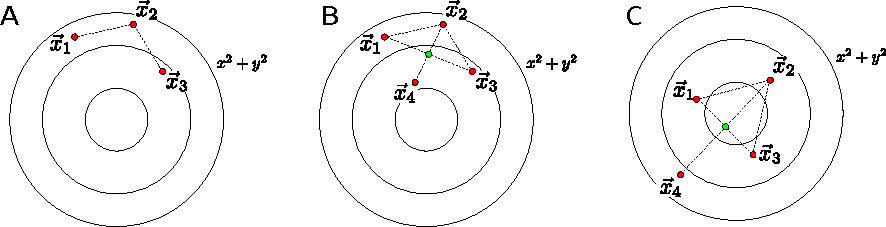
\includegraphics{./simplex.pdf}
\caption{Representação do método simplex de minimização sem derivadas.
(A) Pontos iniciais. (B) Ponto $\vec{x}_4$ gerado na direção de descida
sugerida pelos pontos anteriores. (C) Ponto $\vec{x}_4$ é
insatisfatório.}\label{simplex}
\end{figure}
De acordo com a Figura~\ref{simplex}A, o valor da função em $\vec{x}_1$ é
menor que em $\vec{x}_2$, e o valor da função em $\vec{x}_3$ é o menor
de todos. $\vec{x}_2$ é o pior dos três pontos. 
Ou seja, a função parece diminuir nas direções $\vec{d}_{21}=\vec{x}_1-\vec{x}_2$ e
$\vec{d}_{23}=\vec{x}_3-\vec{x}_2$.

Agora vamos calcular a função em um novo ponto $\vec{x}_4$. Onde deve
ser escolhido esse novo ponto? Ou seja, para onde devemos {\it andar}
sobre a superfície da função, em função do conhecimento adquirido na
avaliação dos pontos anteriores? 

O método simplex consiste em calcular o ponto médio da posição dos $N-1$ melhores
pontos (neste caso, $N=3$), e espelhando o pior ponto em relação a esse
ponto médio. Este procedimento está ilustrado na Figura~\ref{simplex}B.
O novo ponto, na Figura~\ref{simplex}B, é o ponto $\vec{x}_4$.
Formalmente, portanto, a implementação do simplex em duas variáveis
consiste em:
\begin{enumerate}
\item
Ordenar os pontos de melhor a pior valor de função. Digamos, para
exemplificar, que a ordem é, como na Figura~\ref{simplex}A, 
$f(\vec{x}_2) > f(\vec{x}_1) > f(\vec{x}_3)$.
\item
Calcular $\vec{x}_{\text{médio}} = \frac{1}{2}\left(\vec{x}_1+\vec{x}_3\right)$
\item
Espelhar $\vec{x}_2$ em relação a $\vec{x}_\text{médio}$. Ou seja,
calcular
$\vec{x}_4=\vec{x}_2 + 2(\vec{x}_\text{médio}-\vec{x}_2)$
\item
Voltar ao passo 1.
\end{enumerate}
Este novo ponto $\vec{x}_4$ está representado na Figura~\ref{simplex}B.
Podemos ter sorte e a função efetivamente diminuir nesse novo ponto em
relação a algum dos pontos anteriores (como acontece no desenho, onde
ele é o melhor de todos). Neste caso, o novo ponto é aceito,
substituindo o pior dos três pontos anteriores, e recomeça-se o
procedimento.

No entanto, como mostra a Figura~\ref{simplex}C, o novo ponto gerado
pode ser pior que todos os anteriores. Não faz sentido então substituir nenhum
dos pontos. Neste caso, parece ser que passamo por cima de um
vale (na Figura~\ref{simplex}C é efetivamente assim). Por isso, sugere-se fazer uma
``busca linear'' ao longo da linha definida pelos pontos $\vec{x}_2$ e
$\vec{x}_4$. Por exemplo, testando pontos da forma
\[
\vec{x}_5 = \vec{x}_2 + \gamma ( \vec{x}_4 - \vec{x}_2 )
\]
onde $0<\gamma<1$. No nosso exemplo, vamos fazer uma busca pouco
sofisticada. Vamos simplesmente gerar {\it até} 10 pontos aleatórios, nessa
linha, e se conseguirmos um ponto melhor que $\vec{x}_2$, aceitamos esse
ponto e voltamos ao começo. Se não conseguirmos, decretamos todo o
processo como terminado. Além disso, vamos parar se a diferença de
função entre os três pontos em uma iteração é menor que uma precisão
desejada. 

O código deste programa vai ser o maior que colocaremos aqui,
diretamente, no tutorial. Tente entender o código em função da descrição
acima, e tire todas as suas dúvidas com o professor. As próximas etapas
consistirão em substituir as funções neste código por coisas mais
interessantes. Em seguida, pararemos de reinventar a roda, porque há
pessoas que escreveram códigos melhores que os nossos, e nós podemos
utilizar esses códigos na forma de subrotinas sempre que for
conveniente.  

O código do método simplex, como descrito acima, é:

\codefile{./codes/simplex.f90}

\begin{ex}
\item
Modifique o programa para minimizar a função $x^2 + \sen(y)$.
\item
Modifique o programa para minimizar a função $x^2 + y^2 + z^2$. Cuidado
com as dimensões dos vetores, inicializações, etc!
\item
Na forma como foi descrito e implementado, o novo ponto testado está
sempre a uma distância dos pontos anteriores semelhante às distâncias
entre eles. Você pode ter notado isso na lentidão em que o método
converge quando a função está próxima da solução. Modifique o programa
de tal forma que, desde o início, os pontos gerados estejam próximos, e
observe o comportamento.
\item
A observação anterior mostra que, se os pontos são próximos, 
o caminhar sobre a função pode ser muito
lento. Nada nos impede de tentar algo mais ousado. Pense o que poderia
ser modificado no método para admitir um caminhar mais rápido sobre a
superfície da função. Tente implementar suas ideias.  
\end{ex}
\begin{ex}
\item
Este método depende da ordenação dos pontos de melhor a pior, do ponto
de vista do valor da função. O método implementado aqui se chama
``método da inserção'', e é um dos mais simples. Entenda o que o método
faz.
\item
Separe o algoritmo de ordenação do resto do programa, na forma de uma 
subrotina. 
\end{ex}

\section{Aplicando a otimização a um problema ``real''}
\label{real2d}

Nas primeiras partes deste tutorial, aprendemos a fazer uma simulação de
uma cinética química. Estas simulações, foi discutido, podem ser úteis
para validar propostas cinéticas, por comparação com resultados
experimentais. Por exemplo, seja a nossa reação 
\[
\ch{A} \xrightleftharpoons[k_{-1}]{k_1} \ch{B}.
\]
A representação acima é uma proposta para o mecanismo dessa reação, que
deve ocorrer em uma etapa em ambos os sentidos. Suponha que essa reação
foi estudada experimentalmente, o que significa obter, ao longo do
tempo, as concentrações de A e B. Neste caso, ao obter uma obtemos as
duas, por balanço de massa. Queremos, então, verificar se o mecanismo
proposto é razoável e determinar as constantes de velocidade. Em um caso
simples como este, em que a fórmula analítica da concentração em
função do tempo é conhecida, 
\[
[\ch{A}] = \frac{k_1-k_{-1}e^{-(k_1+k_{-1})t}}{k_1+k_{-1}}[\ch{A}_0]
\]
basta ajustar essa fórmula aos
dados experimentais. Isto pode ser feito com qualquer programa de
ajustes não-lineares. Se o ajuste for bom, acreditamos que o mecanismo
deve ser correto e, entre os parâmetros do ajuste, teremos as constantes
de velocidade. 

Se, por outro lado, a reação é um pouco mais complicada (como no exemplo
da ozônio atmosférico, que ilustramos antes), não há uma solução
analítica para a cinética reacional. Desta forma, só é possível comparar
os dados experimentais com a proposta cinética pela realização de
simulações. Uma vez feita uma simulação, podemos comparar as
concentrações medidas em cada momento do tempo, com as concentrações
previstas pelas simulações nos mesmos tempos. Assim, da mesma forma como
se faz com um ajuste, comparamos a validade do mecanismo proposto. 

No entanto, para fazer a simulação, precisamos das constantes de
velocidade. Em princípio podemos não saber quanto valem. Aliás, este é o
caso mais interessante, em que é necessário validar o mecanismo e, ao
mesmo tempo, determinar estas constantes. Neste caso, portanto, é
necessário:
\begin{enumerate}
\item
Fazer várias simulações com constantes de velocidade distintas.
\item
Comparar o resultado (concentrações em função do tempo) em cada
simulação, com o dado experimental.
\item
Verificar se há um conjunto de constantes de velocidade que explica bem
o resultado experimental, dando suporte ao mecanismo proposto.
\end{enumerate}
Naturalmente, a forma inteligente de fazer essas várias simulações, com
diferentes constantes de velocidade, não é testar qualquer coisa. A
forma inteligente é usar um {\it método de otimização} para {\it variar
as constantes de velocidade} de forma a  {\it
minimizar a discrepância} entre o resultado da simulação e o resultado
experimental.

O que vamos fazer aqui é transformar aquele programa Simplex, que
minimiza uma função sem graça, em um programa que minimiza a
discrepância entre um resultado de uma simulação e um dado
``experimental'', de tal forma a obter as constantes de velocidades
corretas. 

\subsection{Resultado experimental}

O ``resultado experimental'', neste caso, será o resultado de uma
simulação feita com seu programa que simula a reação unimolecular
reversível (programa {\tt sim2} da Seção~\ref{sims}). Escolha
concentrações iniciais para os compostos A e B e constantes de
velocidade, e faça uma simulação. Estas concentrações iniciais você vai
usar como parâmetros de entrada no programa que faremos a seguir, porque
é um parâmetro controlado pelo pesquisador. As constantes de velocidade
nós vamos {\it determinar}, como se fossem parâmetros desconhecidos.

\begin{ex}
\item
Escolha um conjunto de parâmetros (concentrações iniciais e constantes
de velocidade), e execute o programa {\tt sim2} da Seção~\ref{sims}.
Guarde o arquivo de saída, que contém as concentrações em função do
tempo.
\end{ex}

\subsection{Comparação com a simulação}

Das simulações acima, você vai ter uma lista de concentrações para
diferentes tempos. Como nossa reação, aqui, é simples, vamos nos
concentrar na concentração de um dos reagentes, [A]. A simulação do item
anterior gerou uma séria de valores de para [A], para diferentes
instantes do tempo. Esqueça que esses valores vieram de uma simulação, e
imagine que foram obtidos experimentalmente. De agora em diante,
chamaremos esses valores de concentrações experimentais. As
concentrações experimentais formam uma lista, ([A](1),[A](2),....), em
que [A](N) é a concentração de A no N-ésimo instante de tempo (a
diferença de tempo entre duas concentrações consecutivas depende do
passo de tempo da sua simulação acima). 

Agora, vamos fazer uma simulação da mesma reação (lembre-se, os dados
que temos são {\it experimentais}), e comparar com os dados
experimentais. Para isso, vamos definir uma função de comparação, que é
a soma do quadrado das diferenças entre os dados experimentais e os
simulados: 
\begin{code}
  f = 0.d0
  do i = 1, N
    f = f + (aexp(i)-asim(i))**2
  end do
\end{code}
onde {\tt aexp} é um vetor que contém os dados experimentais, e {\tt
asim} é o resultado da simulação. Ou seja, para cada uma dos {\tt N}
instantes de tempo em que há medidas experimentais, calculamos o
quadrado diferença da previsão da simulação com o dado experimental.
Somamos todas essas diferenças para avaliar quão parecidos são os dois
conjuntos de dados.
\begin{ex}
\item
Faça um programa que leia os resultados ``experimentais'', faça uma
simulação com outro conjunto de constantes de velocidades (mesmas
concentrações iniciais), e calcule a função acima. Reporte a
similaridade entre o resultado da simulação e o resultado experimental.
Faça um teste usando o conjunto de constantes de velocidade {\it
corretos}, para validar seu programa. 
\end{ex}

\subsection{Descobrindo as constantes de velocidade}

O programa que você fez na seção anterior deve ler os resultados
experimentais, fazer uma simulação, e calcular a similaridade dos dois
resultados. Ou seja, dado um conjunto de constantes de velocidade,
avalia a qualidade da sobreposição dos dados experimentais com a
simulação. Esta qualidade de sobreposição será a nossa {\it função
objetivo}. Ou seja, voltando aos nosso métodos de otimização, tudo que
envolve este último programa será objeto da subrotina que calcula a
função. 
\begin{ex}
\item
Transforme o seu programa, acima, em uma subrotina, que se chame {\tt
computef}. 
\item
Substitua a subrotina que calcula a função no programa Simplex da Seção~\ref{sec:simplex}. 
Cuidado com os nomes das variáveis, porque as constantes
de velocidade tomarão o lugar do vetor {\tt x}. 
\item
Seu programa consegue descobrir as constantes de velocidade corretas,
partindo de chutes aleatórios?
\end{ex}
Note que, agora, a {\it avaliação da função envolve uma simulação}. Isto
é bastante sofisticado.  

\subsection{Refinamentos do programa}

Se você não foi mais esperto do que o previsto, seu programa da seção
anterior deve estar lendo os dados experimentais todas as vezes que
chama a subrotina {\tt computef}. Ler o arquivo do disco rígido todas as
vezes que a função é calculada é muito ruim. Provavelmente seu programa
demora mais tempo fazendo isso que calculando outras coisas. Nesta
seção, vamos mostrar como fazer isso melhor, e aproveitar para
introduzir outras estruturas de programação que são fundamentais em
programas mais complexos.    

Nós queremos que o programa leia só uma vez os dados experimentais.
Portanto, essa leitura não pode estar dentro da subrotina {\tt
computef}, que é {\it chamada} muitas vezes. A leitura deve estar no
programa principal. A leitura de dados é alguma coisa da forma 
\begin{code}
open(10,file='sim2.dat')
do i = 1, N
  read(10,*) aexp(i)
end do
close(10)
\end{code}
A leitura preenche o vetor {\tt aexp}, que contém as concentrações do
reagente A para cada instante experimental. Esse mesmo vetor deve ficar
disponível dentro da subrotina {\tt computef}, sem precisar ser
novamente preenchido todas as vezes que esta subrotina for chamada. Para
isso, servem as estruturas dos {\it módulos}. Os módulos são usados da
seguinte forma:
\begin{enumerate}
\item
Antes do programa principal, define-se um módulo que contém as variáveis
de interesse. por exemplo:
\begin{code}
module reaction
  double precision :: aexp(1000)
end module reaction
\end{code}
\item
No programa principal, antes da declaração das variáveis, e antes mesmo
do {\tt implicit none}, declaramos que vamos {\it usar} esse módulo:
\begin{code}
program simplex
  use reaction
  implicit none
  ...
\end{code}
As variáveis que foram definidas no módulo {\it não} podem ser novamente
declaradas no programa principal. 
\item
Por fim, dentro da subrotina {\tt computef}, que vai precisar desses
dados, também declaramos que vamos usar as variáveis definidas no
módulo:
\begin{code}
subroutine computef(x,f)
  use reaction
  implicit none
  ...
\end{code} 
\end{enumerate}
A leitura dos dados, agora, pode ser feita no programa principal, em
qualquer lugar, antes da primeira chamada à subrotina {\tt computef}. 
Naturalmente, em algum lugar onde não se repita. Esta
leitura vai preencher o vetor {\tt aexp}, que ficará disponível para
todas as rotinas do programa que usam o módulo {\tt reaction}. O módulo
pode conter outros dados da reação, por exemplo, as concentrações
iniciais e o passo de tempo, que são necessários para fazer a simulação
e é natural que sejam parâmetros definidos pelo usuário no programa
principal (ou mesmo lidos de algum arquivo).
\begin{ex}
\item
Modifique o seu programa da atividade anterior de tal forma que todos os
parâmetros que são definidos apenas uma vez e são necessários para o
cálculo da função sejam colocados em um
módulo, que é compartilhado pelo programa principal e pela subrotina.
\end{ex}

O programa Simplex, com todas as modificações desta seção, está
disponível abaixo. Tente fazer tudo antes de ver o resultado. Seu
programa não vai ficar igual a este, e você vai errar várias vezes antes
de chegar a algo que funciona. Isso é normal, e faz parte do
aprendizado, e não só do aprendizado, da própria natureza da
programação, mesmo para quem já tem experiência. A disponibilidade do
código serve principalmente para tirar dúvidas, e aprimorar soluções.
\codelink{./codes/kineticmodel.f90}

\subsection{Usando uma subrotina pronta}

O último grande passo em termos de fundamento de programação que devemos
dar é o uso de uma subrotina ou função que foi escrita por outra pessoa.
Neste caso, vamos usar uma subrotina que implementa o método Simplex com
todo o cuidado, e com variações que o fazem mais eficientes. Há milhares
de subrotinas de cálculo numérico programadas em Fortran que podem ser
utilizadas gratuitamente. Uma busca na internet permite encontrar muitas
coisas boas. A subrotina que vamos usar foi encontrada no google mesmo,
buscando por ``simplex fortran 90''. Todo algoritmo relativamente
sofisticado já foi implementado por alguém.

A código que vamos usar está no arquivo {\tt NelderMeadMinimizer.f90}, e
foi escrito originalmente por David E. Shaw. Por curiosidade, D. E. Shaw
era um cientista da computação da Universidade de Columbia, que
abandonou a carreira acadêmica para se dedicar a ganhar dinheiro na
bolsa de valores usando métodos de otimização de riscos. Ficou
bilionário e entediado, e criou uma instituição de pesquisa dedicada à
bioquímica computacional, na qual desenvolve computadores
especificamente desenhados para simulações de dinâmica molecular (D. E.
Shaw Research). 

A subrotina que vamos usar está disponível aqui:

\begin{center}
\href{http://www.nist.gov/pml/div684/grp03/upload/NelderMeadMinimizer.f90}
{\textcolor{blue}{http://www.nist.gov/pml/div684/grp03/upload/NelderMeadMinimizer.f90}}
\end{center}

Para usar uma subrotina precisamos entender o que ela requer como
parâmetros de {\it entrada} e {\it saída}. Neste caso, você vai notar
que o arquivo possui três subrotinas, chamadas {\tt minimize\_2d}, {\tt
minimize\_1d} e {\tt minim}. 

A subrotina principal, em que o algoritmo simplex está efetivamente
implementado, é a {\tt minim}. Leia com cuidado os comentários o
arquivo. Como você vai notar, a subrotina {\tt minim} possui muitos
parâmetros, alguns dos quais não temos muita certeza do que são, sem
conhecer o algoritmo implementado com maiores detalhes. Por causa desta
complexidade, o programador fornece as outras duas subrotinas, {\tt
minimize\_2d} e {\tt minimize\_1d}, que simplificam o uso da subrotina
principal em problemas específicos.

Aqui vamos nos concentrar na subrotina {\tt minimize\_2d}. Como o nome
sugere, está pensada para a minimização de funções de duas variáveis.
Nosso problema da seção~\ref{real2d} é um problema de duas variáveis (as
duas constantes de velocidade). Vamos, então, usar esta subrotina para
resolver aquele problema.

\subsubsection{Subrotina {\tt minimize\_2d}}

A subrotina {\tt minimize\_2d} é bem mais simples que a {\tt minim}. Tem
apenas cinco parâmetros: {\tt X0, FCN, X, F, Info}. Todos estes
parâmetros são fáceis de entender:


$\bullet$ {\tt X0}: é, obviamente, a primeira
aproximação das variáveis (o ponto inicial). Você vai ter que fornecer
este ponto inicial. Note, na subrotina {\tt minimize\_2d}, o que é feito com {\tt X0}.

$\bullet$ {\tt FCN}: como o nome sugere, tem relação com a função. Note que está
declarado de uma forma estranha, como {\tt EXTERNAL~FCN}. Isso significa
que {\tt FCN} não é um vetor ou um número. {\tt FCN} é uma subrotina ou
uma função. Você vai ter que fornecer para a subrotina {\tt
minimize\_2d} o nome de uma subrotina que calcula a função. Isto porque,
dentro do método simplex, esta subrotina vai ser usada. Portanto, a
rotina que você vai fornecer precisa ser consistente (nos parâmetros de
entrada e saída) com a subrotina que o método espera.
\begin{ex} 
\item
Identifique como o parâmetro {\tt FCN} é passado até a subrotina
principal, {\tt minim} (ele muda de nome, inclusive). Em seguida, leia
os comentários da subrotina {\tt minim} para entender como tem que ser
esta subrotina ou função, do ponto de vista de seus parâmetros de
entrada e saída.
\item
Retome o programa da seção~\ref{real2d}, e veja se sua subrotina de
cálculo da função é consistente com o que é necessário para este novo
programa. Se não for, ajuste os parâmetros de entrada e saída para que
seja (lembre-se, os nomes das variáveis não são importantes, o que
importa é o tipo e a ordem em que são passados). 
\end{ex}

$\bullet$ {\tt X}: Este vetor vai conter a solução encontrada pelo
método simplex. Note como ele está declarado em {\tt minimize\_2d}, e
como ele é passado entre as outras subrotinas.  

$\bullet$ {\tt F}: como o nome sugere, este será o valor da função, ao
final da otimização. Confira isso seguindo as passagens entre as
subrotinas, e os comentários da rotina {\tt minim}.

$\bullet$ {\tt Info:} Muitas subrotinas possuem uma variável como esta,
que indicará se alguma coisa não funcionou como deveria. Note que é um
número inteiro, e veja nos comentários de {\tt minim} o significado de
cada um dos valores de retorno.

\subsubsection{Preparando nosso programa para usar {\tt minimize\_2d}}

O nosso programa, agora, vai ser bastante mais simples que os
anteriores, porque toda a parte complicada está implementada na
subrotina que pegamos pronta. Vamos precisar apenas:
\begin{enumerate}
\item
Declarar corretamente todas as variáveis que serão usadas,
de forma consistente com as subrotinas que vamos usar. 
\item
Adaptar a subrotina que calcula a função, se necessário. O que inclui
ler os parâmetros do modelo, da mesma forma que fizemos anteriormente.
\item
Gerar um ponto inicial para as variáveis.
\item
Chamar a adequadamente a subrotina {\tt minimize\_2d} com e verificar
qual foi o resultado.
\end{enumerate}

A primeira tarefa consiste, então, em declarar corretamente as
variáveis, de acordo com o que a subrotina {\tt minimize\_2d} requer.
São alguns inteiros e vetores de dupla precisão ({\tt double~precision}
e {\tt REAL*8} são sinônimos). Além disso, como a subrotina que você vai
fornecer para calcular a função vai, também, ser um parâmetro, ela
precisa ser declarada, como foi feito na rotina {\tt minimize\_2d}. Seu
programa vai precisar ter uma declaração do tipo
\begin{code} 
external computef
\end{code}
onde {\tt computef} é o nome da subrotina que você programou para
calcular a função. 

\begin{ex}
\item
Copie seu programa se seção~\ref{real2d} em um novo arquivo. Remova tudo
o que consistia no método simplex propriamente dito, com seu método
iterativo. Coloque a chamada à subrotina minimize\_2d, a ajuste todas as
declarações de variáveis.
\end{ex}

O seu código, que chamarei aqui {\tt modelab.f90} pode ser compilado
juntamente com a rotina que você pegou na internet, usando:
\begin{center}
{\tt gfortran -o modelab modelab.f90 NelderMeadMininimizer.f90}
\end{center}

Tente fazer seu programa funcionar. Com um detalhe: dentro da subrotina
{\tt minimize\_2d} há um parâmetro chamado {\tt IPrint}, que por padrão
está definido como $-1$. Altere este valor, por exemplo para $+1$, você
faz com que mais coisas sejam escritas pela subrotina {\tt minim} no
processo iterativo. Isto é interessante para ver o que está
acontecendo. 

A solução para toda esta atividade está disponível aqui:

\codelink{./codes/modelab.f90}


\end{document}


